\documentclass[compress]{beamer}
\usepackage{ifthen,verbatim}

\title{iCSA08 plan: Muon Alignment (HIP)}
\author{Jim Pivarski, Alexei Safonov}
\institute{Texas A\&M University}
\date{ 1 April, 2008}

\newcommand{\isnote}{}
\xdefinecolor{lightyellow}{rgb}{1.,1.,0.25}
\xdefinecolor{darkblue}{rgb}{0.1,0.1,0.7}

%% Uncomment this to get annotations
%% \def\notes{\addtocounter{page}{-1}
%%            \renewcommand{\isnote}{*}
%% 	   \beamertemplateshadingbackground{lightyellow}{white}
%%            \begin{frame}
%%            \frametitle{Notes for the previous page (page \insertpagenumber)}
%%            \itemize}
%% \def\endnotes{\enditemize
%% 	      \end{frame}
%%               \beamertemplateshadingbackground{white}{white}
%%               \renewcommand{\isnote}{}}

%% Uncomment this to not get annotations
\def\notes{\comment}
\def\endnotes{\endcomment}

\setbeamertemplate{navigation symbols}{}
\setbeamertemplate{headline}{\mbox{ } \hfill
\begin{minipage}{5.5 cm}
\vspace{-0.75 cm} \small
\end{minipage} \hfill
\begin{minipage}{4.5 cm}
\vspace{-0.75 cm} \small
\begin{flushright}
\ifthenelse{\equal{\insertpagenumber}{1}}{}{Jim Pivarski \hspace{0.2 cm} \insertpagenumber\isnote/\pageref{numpages}}
\end{flushright}
\end{minipage}\mbox{\hspace{0.2 cm}}\includegraphics[height=1 cm]{../cmslogo} \hspace{0.1 cm} \includegraphics[height=1 cm]{../tamulogo} \hspace{0.01 cm} \vspace{-1.05 cm}}

\begin{document}
\frame{\titlepage}

%% \begin{notes}
%% \item This is the annotated version of my talk.
%% \item If you want the version that I am presenting, download the one
%% labeled ``slides'' on Indico (or just ignore these yellow pages).
%% \item The annotated version is provided for extra detail and a written
%% record of comments that I intend to make orally.
%% \item Yellow notes refer to the content on the {\it previous} page.
%% \item All other slides are identical for the two versions.
%% \end{notes}

\begin{frame}
\frametitle{Outline}
\Large
\begin{itemize}\setlength{\itemsep}{0.75 cm}
\item Context of start-up alignment
\item Workflows in iCSA08
\item Monitoring and Validation
\item Timeline
\end{itemize}
%% \hspace{-0.83 cm} \textcolor{darkblue}{\Large Outline2}
\end{frame}

\begin{frame}
\frametitle{Overview of alignment procedures}

\vspace{1.2 cm}
\mbox{ } \hfill 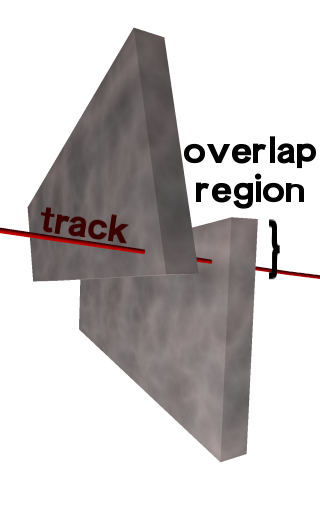
\includegraphics[width=0.15\linewidth]{overlap.png}

\vspace{-3.8 cm}
\begin{itemize}
\item Track-based alignment with HIP

\begin{itemize}
\item \textcolor{darkblue}{``Baseline procedure''} align each chamber (DTs and CSCs) to the tracker
\begin{itemize}
\item uses tracker as an external reference
\item requires at least 10~pb$^{-1}$
\item well-studied procedure
\end{itemize}

\item \textcolor{darkblue}{Beam-halo alignment} align CSCs to each other
\begin{itemize}
\item uses CSC overlap regions (all endcap except ME1/3)
\item relative alignment within each CSC ring
\item internally-aligned rings can be easily aligned to the tracker
\end{itemize}

\item \textcolor{darkblue}{Layer alignment} align CSC layers to layer 1 in each chamber
\begin{itemize}
\item similar procedure, but not limited to overlap regions
\item also possible with beam-halo
\end{itemize}

\item Note that ``beam-halo'' and ``layer'' techniques can both be applied to beam-halo and I.P.\ muons
\end{itemize}

\item Track-based alignment with MillePede
\begin{itemize}
\item see Pablo's talk
\end{itemize}

\item Hardware alignment
\begin{itemize}
\item independent point of comparison, more relevant \mbox{in real-data tests\hspace{-1 cm}}
\end{itemize}

\end{itemize}
\end{frame}

\begin{frame}
\frametitle{Baseline procedure}

\begin{itemize}
\item Tracks are iteratively re-fit with varying hit-weights
\begin{enumerate}
\item loose hit weights in the muon system: project tracks from tracker and align first station
\item tight hit weights in first station: align second station
\item etc.
\end{enumerate}
\item Each chamber is aligned independently of its neighbors
\end{itemize}

\vfill
\begin{columns}
\column{0.6\linewidth}
\begin{itemize}\setlength{\itemsep}{0.25 cm}
\item Test with CRAFT: full tracker and high statistics for top and bottom chambers

\item Maybe test with CRA0T: how essential is our $p_T$ cut? \mbox{(to be studied)\hspace{-1 cm}}

\item Estimate 1~million \mbox{muons in MB0 (good),\hspace{-2 cm}} \\ 10k muons in ME1/3 (fair)
\end{itemize}

\vspace{0.3 cm}\mbox{ }

\column{0.5\linewidth}
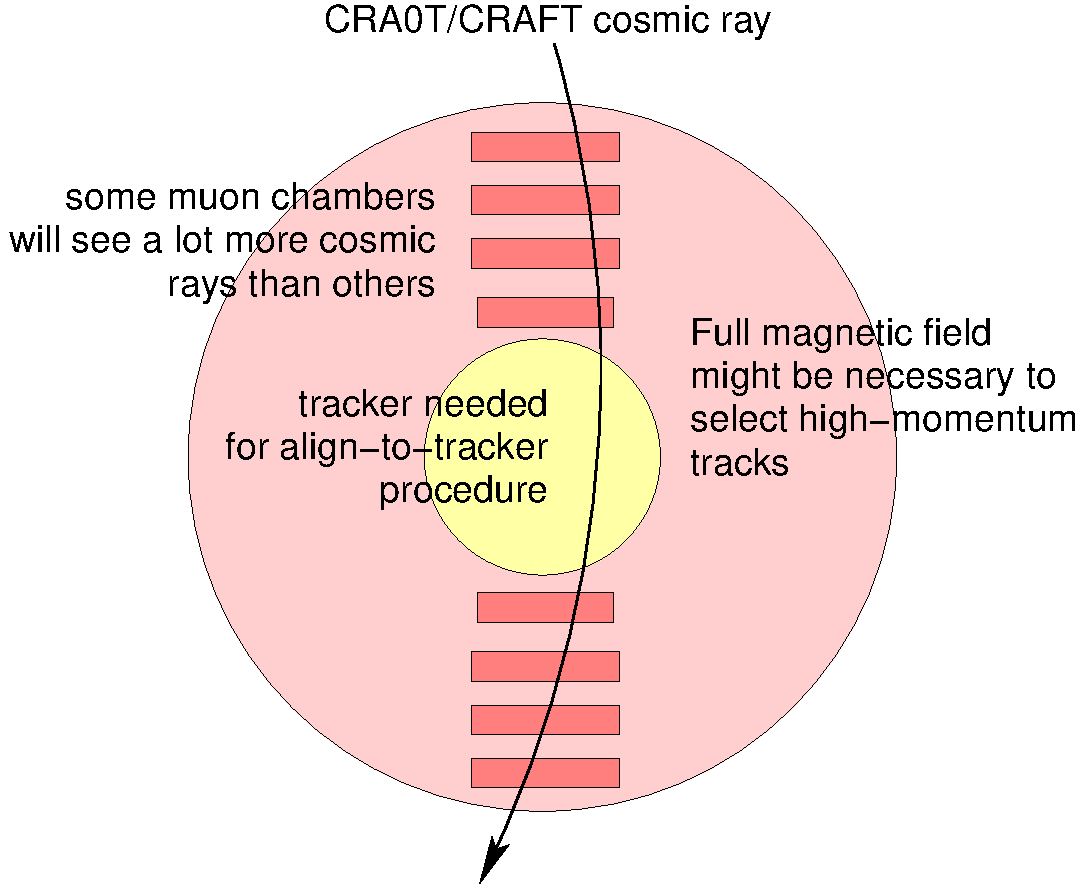
\includegraphics[width=\linewidth]{craft.pdf}
\end{columns}
\end{frame}

\begin{frame}
\frametitle{Beam-halo/layer alignment}

\vspace{-0.5 cm}
\begin{center}
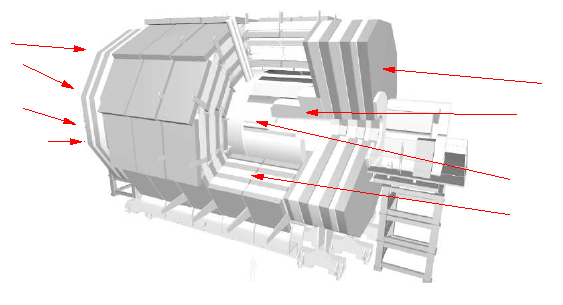
\includegraphics[width=0.4\linewidth]{beam-halo_schematic.png} \hspace{0.5 cm} 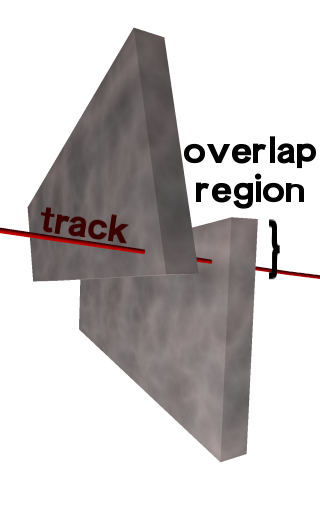
\includegraphics[width=0.15\linewidth]{overlap.png}
\end{center}

\vspace{-0.5 cm}
\begin{itemize}
\item Beam-halo may be a good source of horizontal muons before first collisions
\item Tracks passing through overlap region link pairs of chambers without uncertainty from multiple scattering
\item Specially-configured HIP procedure aligns chambers to each other within CSC rings
\item Small number of I.P.\ muons ($\sim$0.2~pb$^{-1}$) aligns \mbox{rings to tracker\hspace{-1 cm}}
\end{itemize}

\vfill
Beam-halo rate is very uncertain (simulation suggests we'll have
enough muons, but uncertainty quoted as factor of 100)

\vfill
Same technique can be applied to low-energy I.P.\ muons
\end{frame}

\begin{frame}
\frametitle{Workflows in iCSA08}

\begin{enumerate}\setlength{\itemsep}{0.25 cm}
\item Baseline alignment with $W \to \mu\nu$ (10~pb$^{-1}$)
\item Baseline alignment with realistic soup (10~pb$^{-1}$)
\item CSC ring alignment with soup (1 or 10~pb$^{-1}$?)
\item CSC ring alignment with beam-halo ($\sim$1 million overlaps?)
\item CSC layer alignment with soup (1 or 10~pb$^{-1}$?)
\item CSC layer alignment with beam-halo ($\sim$1 million muons?)
\end{enumerate}

\vfill
\textcolor{darkblue}{\small (1)} and \textcolor{darkblue}{\small (2)} are minimal goals

\vfill
Other workflows may be labeled ``minimal goals'' when their parameters are better understood
\end{frame}

\begin{frame}
\frametitle{1{\small \&}2. Baseline workflow}

\begin{itemize}\setlength{\itemsep}{0.5 cm}
\item $W\to\mu\nu$ or soup obtained via ALCARECOMuAlZMuMu stream
\item Procedure takes about 10 hours on 50 CAF nodes
\item Temporarily requires 18~GB on CAF mass storage

\vspace{0.1 cm}
\begin{enumerate}\setlength{\itemsep}{0.2 cm}
\item Select non-scattering tracks from ALCARECOMuAlZMuMu stream, placing a filtered copy on CAF mass storage
\item Align DT wheels and CSC rings
\item Align all chambers in automated procedure
\end{enumerate}
\end{itemize}

\vfill
I'm debugging baseline-procedure scripts on the CAF right now \\ (in 1\_6\_7 with back-ported 2\_0\_X features)

\vfill
Will be tested in 1\_8\_X samples
\end{frame}

\begin{frame}
\frametitle{3{\small \&}4. CSC ring workflow}

\begin{itemize}
\item Soup passed through ALCARECOMuAlOverlaps; \\ beam-halo through ALCARECOMuAlBeamHaloOverlaps
\item Also needs a temporary copy, split by station with the overlap event (8 subsamples)
\item Procedure to be studied in detail this month: current estimate of needed resources:
\begin{itemize}
\item 1 or 10~pb$^{-1}$ ($\sim$5\% of events with endcap \mbox{muons have overlaps)\hspace{-1 cm}}
\item 10's of GB temporarily on CAF mass storage
\item approximately 250 CPU-hours
\end{itemize}
\item ALCARECOMuAlOverlaps will be tested in 1\_8\_X samples, beam-halo needs to be tested independently
\end{itemize}

\vfill
\hspace{-0.83 cm} \textcolor{darkblue}{\Large 5{\small \&}6. CSC layer workflow}

\begin{itemize}
\item Similar to the above, but using ALCARECOMuAlZMuMu and ALCARECOMuAlBeamHalo streams
\item No need to split sample or copy to CAF mass storage
\end{itemize}
\end{frame}

\begin{frame}
\frametitle{Monitoring and validation}

Three tools:
\begin{enumerate}
\item Full iteration-by-iteration, job-by-job residuals histograms for diagnostics if there's a mistake
\item Summary hit residuals plots and alignment positions relative to true (MC diagnostic)
\item MuonAlignmentAnalyzer: segment residuals and physics plots ($Z\to\mu\mu$)
\end{enumerate}

\vfill
Validate with MuonAlignmentAnalyzer before and after alignment

\vfill
Watch hit residuals and alignment positions after each iteration, or at the end of the alignment

\vfill
Run MuonAlignmentAnalyzer in re-reconstruction job to make sure that we uploaded the right constants!
\end{frame}

\begin{frame}
\frametitle{Timeline (in blobs)}
\mbox{\hspace{-0.75 cm} 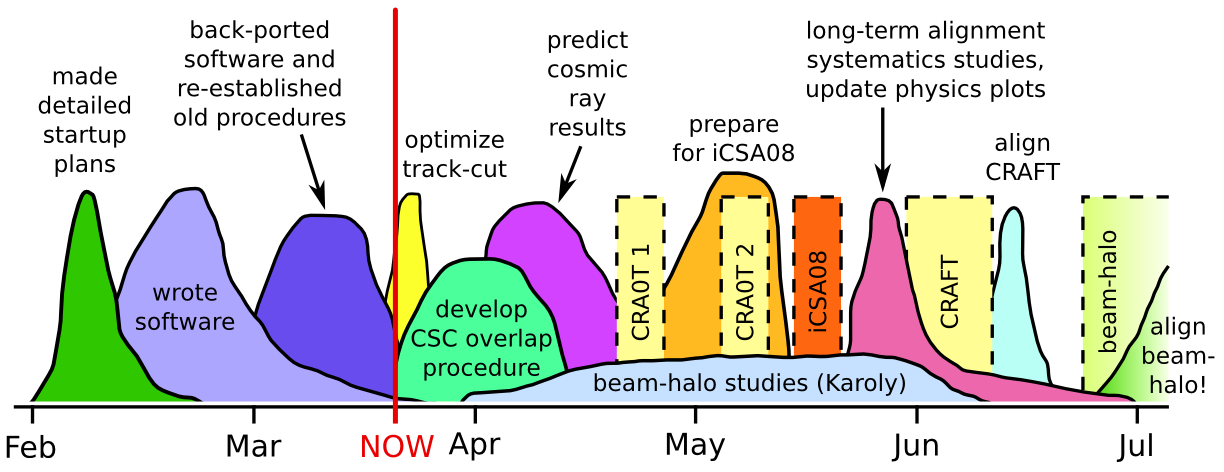
\includegraphics[width=1.12\linewidth]{plan.png}}

\begin{itemize}
\item \textcolor{darkblue}{April:} time to develop the new start-up procedures (set up configuration files)

\item \textcolor{darkblue}{May:} prepare for iCSA08 (tests with 1\_8\_X samples)

\item \textcolor{darkblue}{June:} real-data test with CRAFT data (maybe CRA0T)

\item \textcolor{darkblue}{July:} real alignment with beam-halo
\end{itemize}
\end{frame}

%% \section*{First section}
%% \begin{frame}
%% \begin{center}
%% \Huge \textcolor{blue}{First section}
%% \end{center}
%% \end{frame}

\begin{frame}
\frametitle{Conclusions}

\Large
\begin{itemize}\setlength{\itemsep}{0.5 cm}
\item Well-defined baseline workflow
\item Developing workflows relevant for start-up
\item Resource requests will clarify in the next month
\item Everything to be tested before the iCSA08 event
\item Good lead-in to real-data alignments
\end{itemize}

\label{numpages}
\end{frame}

\end{document}
